\documentclass{article}
\usepackage{natbib}
\usepackage{amsmath}
\usepackage{amssymb}
\usepackage{mathtools}
\usepackage{textcomp}
\usepackage{caption}
\usepackage{float}
\usepackage{subcaption}
\usepackage{graphicx}
\usepackage{ragged2e}
\usepackage{geometry}
\usepackage{tikz}
\usetikzlibrary{positioning}

\newgeometry{
    top = 2.5cm,
    lmargin = 4cm,
    rmargin = 3cm,
    bottom = 2.5cm
}

\title{
  \textbf{
    \huge Technical University of Munich \\ Campus Straubing \\ Faculty of Bioinformatics
        }\\
  \vspace{0,25cm}
  \huge Final report: Research internship \\ Applying Deep Reinforcement Learning to \textit{Lunar Lander}
  }
\author{\huge Krystian Budkiewicz}
\date{\huge 01.12.2022}

\begin{document}
\maketitle
\vspace{4cm}
\tableofcontents

\newpage
\begin{centering}
    \section*{Abstract}
    This document summarizes my 6-week research internship under the assistance of PhD student Jonathan Pirnay at the Faculty of Bioinformatics led by Prof. Dominik Grimm at TUM Campus Straubing, during which I implemented a Deep Q-Algorithm solving the \textit{Lunar Lander} environment. The influence of the learning rate and start, end and termination hyperparameters of the linear epsilon-decay on the score gained by the agent in the environment, as well as the loss-function during the runs were examined.
\end{centering}

\section{Introduction}
In the past decade great progress has been made in the subject of machine learning (ML). One of the most influential steps, has been the usage of neural networks in a subset of ML, reinforcement learning (RL), known as deep reinforcement learning (deep RL), achieving, or in some cases outperforming, human level performance \cite{mnih2015human}. Since then, the usage of deep RL exploded and has become state of the art method for solving complex problems in multiple areas, such as playing video games \cite{mnih2015human}\cite{mnih2013playing}, board games \cite{silver2016mastering}\cite{silver2018general} or optimization of mathematical calculations \cite{fawzi2022discovering}. An advantage of deep RL over rule-based algorithms is their robustness and ability to solve a plethora of different problems with similar approach, rather than being confined to one task, for which the rules have to be explicitly written.

During my internship, I was introduced to the basic ideas of RL and deep learning under the assistance of PhD student Jonathan Pirnay. Using my knowledge gained in both of these topics, I programmed a Deep-Q-Algorithm solving a benchmark toy problem of \textit{Lunar Lander}. This document gives a short introduction to RL, \textit{Lunar Lander} suite and deep Q-learning, and  presents results of my inquiries to variables of the algorithm, as well as their influence on the agent.

\section{Reinforcement Learning}
Reinforcement learning is a subset of ML, which is concerned with the usage of big data-sets for training an artificial intelligence (AI) agent, which solves or optimizes a specific task \cite{lapan2018deep}. The agent resides within an environment, described by a set of states $\mathcal{S}$ it can take, actions $\mathcal{A}$ to exercise and rewards $\mathcal{R}$ to gain. An agent interacts with the environment trough actions $a\in\mathcal{A}$, depending on its current state $s\in\mathcal{S}$ to gain rewards $r\in\mathcal{R}$, in a process called Markov decision process (MDP). From every state, the agent chooses an action and makes a step $t$ within the environment, based on a policy $\pi$:
\begin{equation}
    \label{eqn:policy}
    \pi(s|a)=\mathbb{P}[A_t=a|S_t=s]
\end{equation}
\\
gaining a reward $R_t$ and arriving at a new state $s'$, from which new actions $a'$ can be taken. The amount of reward gained by the agent depends on the next state $s'$ and new actions $a'$ possible from that state. Thus, for every time -step $t$, a return $G_t$ can be calculated:
\begin{equation}
    G_t = R_{t+1}+\gamma R_{t+2}+\cdots = \sum_{k=0}^{\infty}\gamma^{k}R_{t+k+1}
\end{equation}
\\
Every future reward is multiplied with a discount factor $\gamma$, where $\gamma\in[0,1]$, thus decreasing the importance of rewards further in the MDP. The cycle of taking actions from a state, in order to get rewards is repeated until a specific condition is met, after which the episode is terminated.

% v-value and motivation of v(s),q(s,a)
For each state $s$ and state-action pair $(s,a)$, expected return $V^{\pi}(s)$ or $Q^{\pi}(s,a)$ under policy $\pi$ can be calculated, via Bellman equation:
\begin{align}
    \label{eq:bellman}
    V^\pi (s) &= \mathbb{E}_\pi[G_t|s] \\
    Q^\pi (s,a) &= \mathbb{E}_\pi[G_t|s,a]
\end{align}
\\
known as V-value and Q-value respectively. The agent maximizes reward gained after every step, by choosing an action $a$, leading to a new state-action pair $(s',a')$ with the highest Q-value.

Due to the repetitive nature of the task, in which every new state $s'$ becomes the current state $s$, dynamic programming can be implemented to solve the problem. Policy $\pi$ is improved by iteratively applying the Bellman equation to each state, in which the agent resides. Thus, an optimal policy $\pi^*$, which maximizes the amount of reward gained by the agent, after each interaction during the episode, can be found.

\section{Lunar Lander}
The game of \textit{Lunar Lander} is a \textit{Box2D} environment from OpenAI \textit{Gym} library, used as a benchmark for DQN-Algorithms \cite{brockman2016openai}, based on a video game with the same name for a famous 70s game console Atari 2600. The task of the game is to land a lunar lander onto a designated area in the middle of the screen, without crashing the vehicle or leaving the bounds of the environment (Figure \ref{fig:lunarlander}.).

Each episode starts with randomised state-vector $s$ containing eight variables (such as x and y coordinates, angle, velocity, etc.), restricted to a specific, discrete range of values. Based on its current state $s$, the agent can evaluate its position and interact with the environment through four actions $a$: (a) doing nothing or (b, c, d) turning one of the three engines on or off (either left, right or bottom). For every action $a$ chosen by the agent, the environment makes a step (corresponding to a frame within the game) calculating the next state $s'$ and rewarding the agent with a reward $r$ (based on score gained in the game), depending on the action taken and new state $s'$ within the environment. The cycle of evaluating starts all over again, until the episode gets terminated - either due to crashing or turning over the lander, leaving the bounds of the environment, running out of time-steps or successfully landing in the designated area. After each termination, a new episode with randomised state $s$ gets initiated, until the run is over.

The environment is considered solved when the moving average score achieved by the agent in last 100 episodes $\geqslant200$.
\\
\begin{figure}[h]
    \centering
    \includegraphics[width=0.8\linewidth]{figs/lunarlander.jpg}
    \caption{A screenshot of the environment. Lunar lander (violet) descending towards the moon surface (white) onto the designated area between the flags.}
    \label{fig:lunarlander}
\end{figure}

% \pagebreak
\section{Deep Q-Learning}

\subsection{Q-Learning}
In the case of a model-free environment, where sets of states, possible actions, and rewards are unknown, the agent has to resort to trial and error, in order to gain insight about the environment. Only then the optimal behaviour can be determined. The agent gains more knowledge of each state and rewards gained after exercising actions, by saving Q-values in the Q-table, which describes the environment. The agent improves its policy, by using and updating previously created Q-table with every iteration, thus maximising the reward gained after each run.

The initialized Q-table $Q_0$ is a matrix of expected return $Q$ for each action $a$ exercised from each state $s$. In the beginning, nothing is known about the environment, thus $Q_0$ is a matrix of zeros. With each step within the environment, for every state-action pair, the agent "maps out" the environment, by updating the Q-values within the Q-table, using the SARSA-algorithm \cite{rummery1994line}:
\begin{equation}
    Q^{new}(s,a) = Q(s,a) - \alpha \Big( r+\gamma \max_{a} Q(s',a) - Q(s,a) \Big)
\end{equation}
\\
with the learning rate $\alpha$ determining the change of Q-values. After many iterations, the Q-table converges to the true value of each state-action pair $(s,a)$ in the environment, leading to the optimal policy $\pi^*$.

Further improvement to the agents behaviour can be achieved through the implementation of $\varepsilon$-greedy action selection. In such case, the agent chooses a random  or a greedy action, i.e. an action leading to the next state with the highest Q-value, as follows:
\begin{equation}
    \pi(a|s) = \begin{cases}
    \underset{a'}{\text{argmax }}Q^{\pi}(s',a'), & \text{with probability }1-\varepsilon \\
    \text{a random action},     & \text{with probability }\varepsilon
    \end{cases}
\end{equation}
\\
with $\varepsilon\in[0,1]$. The value of $\varepsilon$ is decreased with time, thus steadily increasing the probability of choosing a greedy action. Because of that, an episode can be divided in the exploration phase, where mostly random actions are selected and the exploitation phase, where mostly greedy actions are selected and reward is maximized. This allows the agent to acquire experience and learn a strategy (policy $\pi$) in the exploration phase; then use the best strategy in the exploitation phase, thus reducing the amount of episodes needed to solve an environment.

\subsection{Neural networks}
Artificial neural networks (ANNs) are function approximators, consisting of nodes (perceptrons) arranged in layers, forming a network. Each node from one layer is connected to the another node in the next layer, with a weight vector $\textbf{w}$ and weights $w_j$ describing the strength of the connection between the nodes. These nodes feed forward the input data from an input layer, through inner, hidden layers, to an output layer, giving an output (Figure \ref{fig:nn}.) - where the amount of hidden layers can be varied. For each hidden layer, a dot product of the input vector $\textbf{x}$ and the weight vector $\textbf{w}$ of each node $n$:
\begin{equation}
    \textbf{y} = \textbf{w}\cdot \textbf{x}^{\top} = \sum_{j=1}^{n} \textbf{x}_jw_j
\end{equation}
\\
is calculated. Additionally, every output of the hidden layer $\textbf{y}$ is passed through an activation function, in our case through a rectifying linear unit (ReLU) function:
\begin{equation}
    \text{ReLU}(x) = \max(0,x)
\end{equation}
\\
This sequence of operations is repeated for each hidden layer within the neural network.

\begin{figure}[ht]
    \centering
    \vspace{0.5cm}
    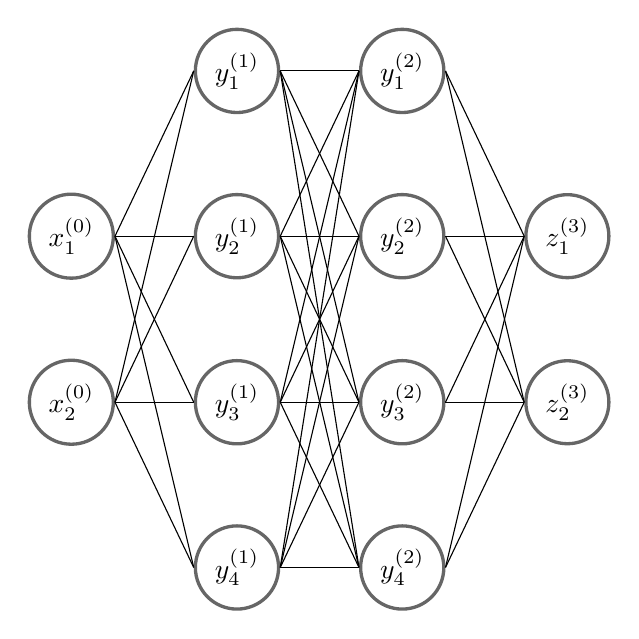
\begin{tikzpicture}[roundnode/.style={circle, draw=black!60, very thick, minimum size=8mm}]
    %Nodes
    \node[roundnode]        (in0)                          {$x_1^{(0)}$};
    \node[roundnode]        (in1)           [below=of in0] {$x_2^{(0)}$};
    \node[roundnode]        (h1)            [right=of in0] {$y_2^{(1)}$};
    \node[roundnode]        (h0)            [above=of h1] {$y_1^{(1)}$};
    \node[roundnode]        (h2)            [right=of  in1] {$y_3^{(1)}$};
    \node[roundnode]        (h3)            [below=of  h2] {$y_4^{(1)}$};
    \node[roundnode]        (g1)            [right=of h1] {$y_2^{(2)}$};
    \node[roundnode]        (g0)            [right=of h0] {$y_1^{(2)}$};
    \node[roundnode]        (g2)            [right=of  h2] {$y_3^{(2)}$};
    \node[roundnode]        (g3)            [right=of  h3] {$y_4^{(2)}$};
    \node[roundnode]        (o0)            [right=of  g1] {$z_1^{(3)}$};
    \node[roundnode]        (o1)            [right=of  g2] {$z_2^{(3)}$};

    %Lines
    \draw (in0.east) -- (h0.west);
    \draw (in0.east) -- (h1.west);
    \draw (in0.east) -- (h2.west);
    \draw (in0.east) -- (h3.west);
    \draw (in1.east) -- (h0.west);
    \draw (in1.east) -- (h1.west);
    \draw (in1.east) -- (h2.west);
    \draw (in1.east) -- (h3.west);
    \draw (h0.east) -- (g0.west);
    \draw (h0.east) -- (g1.west);
    \draw (h0.east) -- (g2.west);
    \draw (h0.east) -- (g3.west);
    \draw (h1.east) -- (g0.west);
    \draw (h1.east) -- (g1.west);
    \draw (h1.east) -- (g2.west);
    \draw (h1.east) -- (g3.west);
    \draw (h2.east) -- (g0.west);
    \draw (h2.east) -- (g1.west);
    \draw (h2.east) -- (g2.west);
    \draw (h2.east) -- (g3.west);
    \draw (h3.east) -- (g0.west);
    \draw (h3.east) -- (g1.west);
    \draw (h3.east) -- (g2.west);
    \draw (h3.east) -- (g3.west);
    \draw (g0.east) -- (o0.west);
    \draw (g0.east) -- (o1.west);
    \draw (g1.east) -- (o0.west);
    \draw (g1.east) -- (o1.west);
    \draw (g2.east) -- (o0.west);
    \draw (g2.east) -- (o1.west);
    \draw (g3.east) -- (o0.west);
    \draw (g3.east) -- (o1.west);
    \end{tikzpicture}
    \caption{An exemplary neural network with 2 inputs, 2 hidden layers consisting of 4 perceptrons each and 2 outputs.}
    \label{fig:nn}
\end{figure}

\newpage
\subsection{Deep Q-learning}
Deep Q-learning combines the usage of action-state function $Q^\pi$ with a feedforward ANN. Instead of improving the agents policy using a Q-table, the behaviour is determined by the ANN, which approximates Q-values of the input and returns the best course of action. In the beginning, the network and its weights is initialized with randomised values. With each iteration, the weights are adjusted in such a way, as to minimize the error between the predicted and true outcomes. Thus, an optimal policy $\pi^*$ can be found.

In Deep Q-learning two separate, local and target neural networks, are used. The local network returns the Q-values based on the current state of the agent, whereas the target network functions as an approximator of the true Q-value of that state. Every time-step, both of these values are compared, in order to measure how good the current prediction model (local network) is. A squared difference of Q-values between both of these networks, known as the loss $\mathcal{L}$, is calculated as follows:
\begin{equation}
    \mathcal{L} = \frac{1}{N}\sum^{N}_{i=1}{(Q_{local}-Q_{target})^2}
\end{equation}
\\
where $N$ is the number of episodes and $Q_{local}$, $Q_{target}$ being Q-values of the respective network.

The network is optimized by setting its weights  to such a value, that minimises the mean-squared error between the approximate and true value of Q, i.e. minimizes the loss $\mathcal{L}$. Given a differentiable function $J(\textbf{w})$ of the parameter vector $\textbf{w}$:
\begin{equation}
    J(\textbf{w}) = \mathbb{E_\pi[\mathcal{L}]}
\end{equation}
\\
the gradient $\nabla_wJ(\textbf{w})$ can be defined as:
\begin{equation}
    \nabla_w J(\textbf{w}) =
    \begin{pmatrix}
        \frac{\partial J(\textbf{w})}{\partial \textbf{w}_n}  \\
        \vdots  \\
        \frac{\partial J(\textbf{w})}{\partial \textbf{w}_n}  \\
    \end{pmatrix}
\end{equation}
\\
By taking steps within the space of $J(\textbf{w})$, with step-size being defined by the learning rate $\alpha$, towards the descending gradient $\nabla_{w}J(\textbf{w})$, in a process called gradient descent, the parameter vector $\textbf{w}$ is adjusted, as follows:
\begin{equation}
    \Delta\textbf{w} = -\alpha\nabla_{w}J(\textbf{w})
\end{equation}
\\
For each weight $w_j$ in $\textbf{w}$, the chain rule is applied:
\begin{equation}
    \frac{\partial w_j}{\partial x}
    = \frac{\partial w_j}{\partial y}\cdot\frac{\partial y}{\partial x}
\end{equation}
\\
adjusting the weights across the layers of the network backwards, based on their change with respect to $\mathcal{L}$, in a process called backpropagation. With every step, the weight gets adjusted to a value that minimizes the loss $\mathcal{L}$; the goal being, finding the minimum of $J(\textbf{w})$, leading to the smallest possible loss $\mathcal{L}$. Thus, every step made by the agent is aligned with the expected one and an optimal policy $\pi^*$ is used. Furthermore, using the $\varepsilon$-greedy action-selection improves agents behaviour, by avoiding local minima in the exploration phase.

Additionally, replay memory - a container storing past experiences - can be implemented \cite{liu2018effects}. In this container of specific size, after each step made by the agent, each state-action pair with its corresponding Q-value achieved in the previous episodes, is saved in a list. In such case, the loss $\mathcal{L}$ is calculated as a squared difference of local network, with the current state $s$ and target network, with a batch of memories from replay. Thus, the agent learns from its own, past behaviour. After the limit of experiences in memory is reached, each old memory is replaced by the most recent one. Similar to the previous case, weights in the neural network get adjusted based on the loss $\mathcal{L}$ with gradient descent and backpropagation.

\newpage
\section{Training procedure}
In preliminary experiments, hyperparameters set during each run were based on those found in code online \footnotemark. After unsuccessful runs these hyperparameters were changed randomly in order to improve agents behaviour, until the agent was able to solve the environment in 5 subsequent runs. Hyperparameters used during these runs are tablified in Table \ref{table:standard}. and will be referred to as "standard parameters" later. Once 5 successful runs were achieved, one of the parameters was changed and its influence on the score achieved by the agent and loss during next 5 runs was noted. Optimization of the neural networks was done using Adam algorithm \cite{kingma2014adam}. The $\varepsilon$-value was decreased linearly from $\varepsilon$-start to $\varepsilon$-end in $\varepsilon$-term episodes.

\begin{table}[ht]
    \caption{Hyperparameters used resulting in first successful runs. Referred to as "standard parameters".}
    \label{table:standard}
    \centering
    \begin{tabular}{cc}
        \hline
        \textbf{Hyperparameter}                      & \textbf{Value} \\
        \hline
        Maximum amount of episodes              & 1500      \\
        Maximum amount of steps                 & 1000      \\
        Batch size                              & 100       \\
        Replay memory size                      & 100000    \\
        Amount of hidden layers                 & 3         \\
        Amount of neurons per hidden layer      & 64        \\
        Target network update frequency         & 6         \\
        Network parameter update factor $\tau$  & 2.5e-3    \\
        Learning rate $\alpha$                  & 2.5e-4    \\
        Discount factor $\gamma$                & 0.99      \\
        $\varepsilon$-start                     & 1         \\
        $\varepsilon$-end                       & 0.01      \\
        $\varepsilon$-term                      & 1000      \\
        \hline
    \end{tabular}
\end{table}

\footnotetext{https://goodboychan.github.io/python/reinforcement_learning/pytorch/udacity/2021/05/07/DQN-LunarLander.html\#Training-Process}

\section{Results and Discussion}

\subsection*{Behaviours of the agent during training}
In order to solve the environment and maximize the reward from given episode the agent tried multiple tactics: (a) hovering with the lunar lander directly or high above the landing area, then slowly descending onto it, (b) dropping fast towards the ground while not breaking the lander, then using one of the engines on the side to push the lander towards the landing area and (c) resembling human-like play-style the most, slowing down from the initial state and descending in a swing-like motion towards the landing area.

During multiple training cycles the agent showed similar behaviours, which resulted in achieving lower scores, such as not slowing down enough from the starting condition and crashing the lander into the ground, flipping the lander over, not solving the environment in the given time (steps), not turning the engines off while on the landing platform or getting out of the environments bounds, thus either terminating the episode (in the case of crashing and flipping over) or achieving a huge negative score.

\newpage
\subsection*{Linear $\varepsilon$-decay}

\subsubsection*{$\varepsilon$-start}
Hyperparameter $\varepsilon$-start is the value of $\varepsilon$ with which the first state gets initialized.

Smaller $\varepsilon$-start lead to smaller probability of taking a random action by the agent, thus increasing the mean score, starting exploitation phase and solving the environment earlier - $\varepsilon$-start = 0.7 being the best value found (Figure \ref{fig:start}.). Also, smaller $\varepsilon$-start tend to minimise the loss-function across the episode faster than values closer to 1 (Figure \ref{fig:start_loss}.), due to the smaller slope of the $\varepsilon$-decay.

\subsubsection*{$\varepsilon$-end}
Hyperparameter $\varepsilon$-end is the value of $\varepsilon$ which remains constant  until the termination of the run after the episode defined by $\varepsilon$-term has been achieved.

Small $\varepsilon$-end lead to faster increase of score during the latter part of the episode (Figure \ref{fig:end}.). After termination of $\varepsilon$, smaller $\varepsilon$-end tend to start exploitation phase faster, thus leading to a plateau in score. Increasing $\varepsilon$-end to an optimum leads to faster solving of the environment by the agent - $\varepsilon$-end = 0.05 being the best value found.

\subsubsection*{$\varepsilon$-term}
Termination of $\varepsilon$ at the episode $e$, is the episode $e$ at which $\varepsilon$-end is reached.

Bigger $\varepsilon$-term increase the time-duration of exploration phase of the agent and lead to later increase of score in latter parts of the episode - $\varepsilon$-term = 1200 being the best value found (Figure \ref{fig:term}.). Because $\varepsilon$-term sets at which episode $\varepsilon$-end is reached, it also sets the steepness of the $\varepsilon$-decay and defines when exploitation phase starts, thus shifting the "take-off" of the score during the episode, with bigger values allowing for longer exploration of the environment.

\subsection*{Learning rate $\alpha$}
Learning rate $\alpha$ determines the step size at each iteration, towards minimizing loss.

Decreasing the value of $\alpha$ increased the amount of episodes needed to solve the environment - $\alpha = 5e-4$ being the best value found (Figure \ref{fig:lr}.). Smaller learning rates, combined with fast $\varepsilon$-decay and small $\varepsilon$-end, disallow the agent to explore new possibilities within the environment after $\varepsilon$-end is reached. Because of that, the agent sticks with the best policy learned up to $\varepsilon$-term, resulting in stagnation of score further in the run, with only occasional variations. Slower $\varepsilon$-decay could yield better results by allowing the agent to explore for longer. Also, smaller learning rates increase average loss during exploration phase during an episode (Figure \ref{fig:lr_loss}.).

\newpage
\begin{figure}[H]
    \begin{subfigure}{0.5\linewidth}
        \centering
        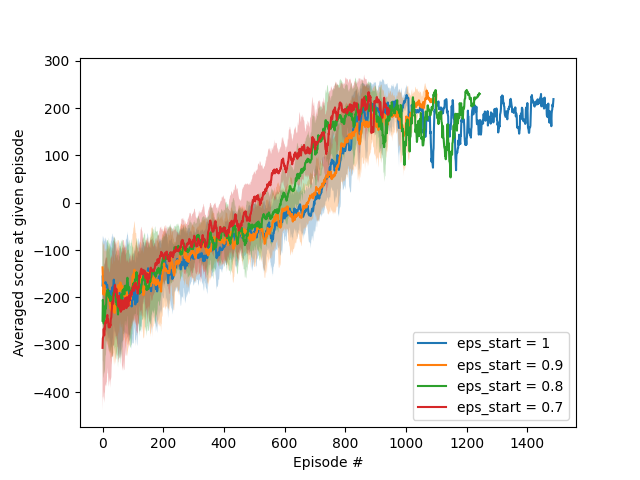
\includegraphics[width=\linewidth]{figs/EPS_START.png}
    \end{subfigure}
    \quad
    \begin{subfigure}{0.5\linewidth}
        \centering
        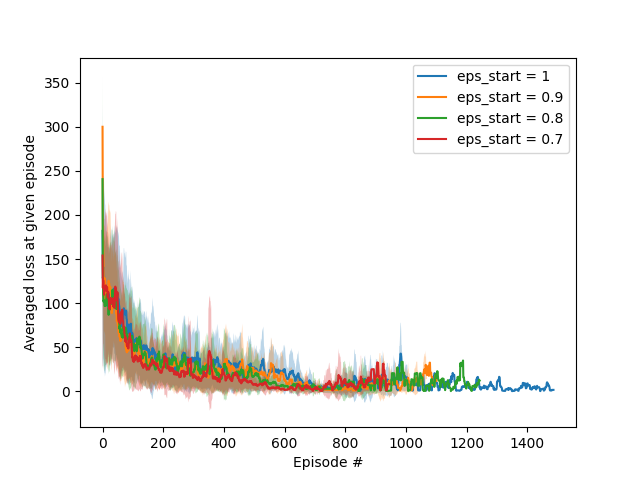
\includegraphics[width=\linewidth]{figs/EPS_START(loss).png}
    \end{subfigure}
    \begin{subfigure}{0.5\linewidth}
        \centering
        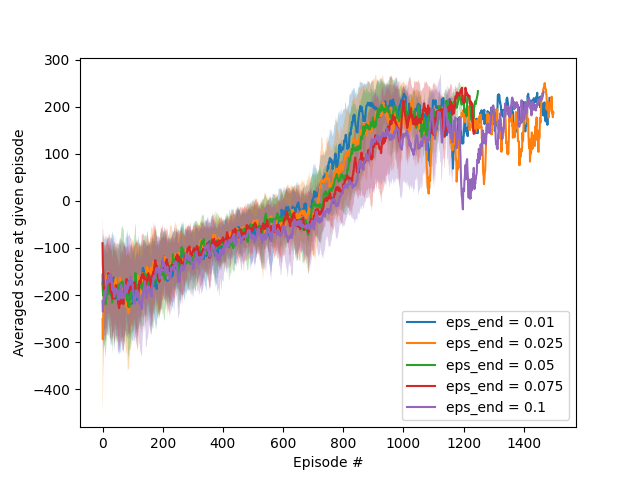
\includegraphics[width=\linewidth]{figs/EPS_END.png}
    \end{subfigure}
    \quad
    \begin{subfigure}{0.5\linewidth}
        \centering
        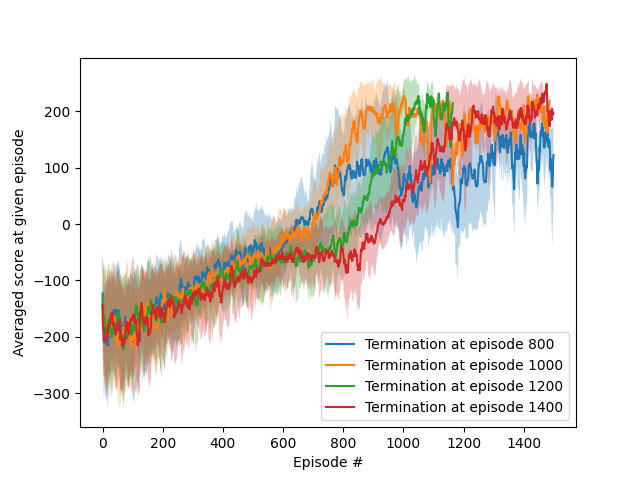
\includegraphics[width=\linewidth]{figs/EPS_TERM.png}
    \end{subfigure}
    \begin{subfigure}{0.5\linewidth}
        \centering
        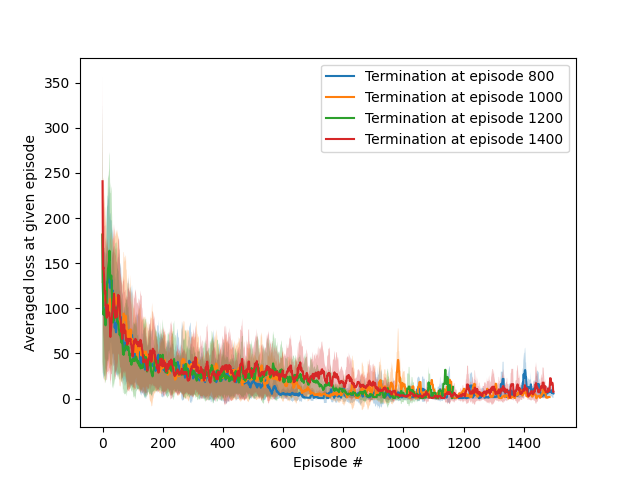
\includegraphics[width=\linewidth]{figs/EPS_TERM(loss).png}
    \end{subfigure}
    \quad
    \begin{subfigure}{0.5\linewidth}
        \centering
        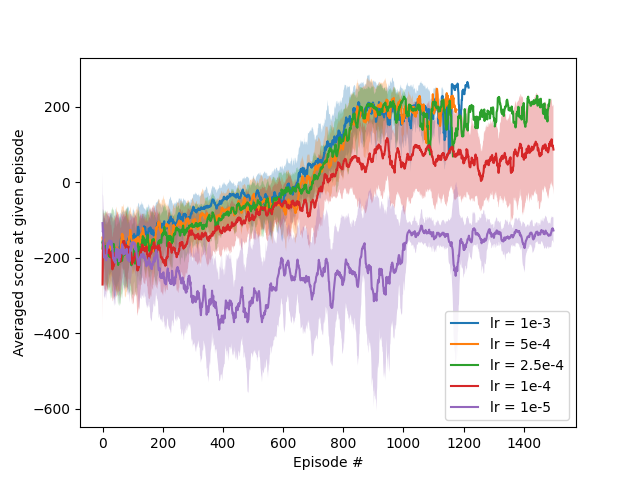
\includegraphics[width=\linewidth]{figs/LR.png}
    \end{subfigure}
    \begin{subfigure}{0.5\linewidth}
        \centering
        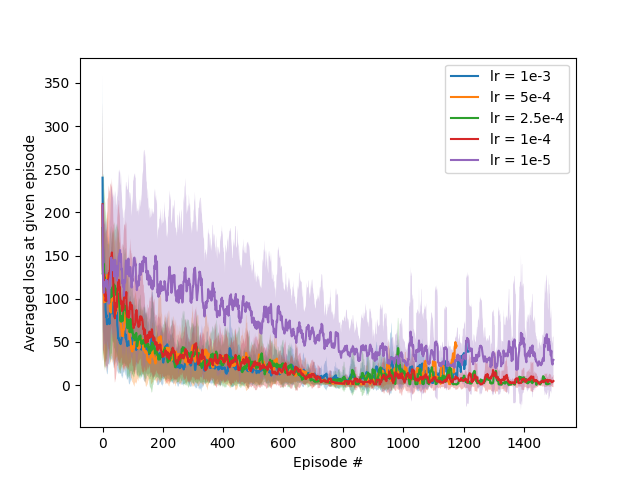
\includegraphics[width=\linewidth]{figs/LR(loss).png}
    \end{subfigure}
    \caption{The influence of learning rate $\alpha$, $\varepsilon$-start, $\varepsilon$-end and $\varepsilon$-term on the average moving score and loss gained by the agent during the run. Shades denote standard errors.}
    \label{fig:results}
\end{figure}

\newpage
\addcontentsline{toc}{section}{Methods}
\section*{Methods}
The deep Q-algorithm was written in \textit{Python} (v. 3.9) with \textit{PyTorch} (v. 1.12.1) and \textit{NumPy} (v. 1.23.3) libraries, as well as certain functions from \textit{collections} library. The \textit{Lunar Lander} environment was imported from \textit{Gym} (v. 0.26.1) library. The code is available on GitHub (https://github.com/kbudkiewicz/research-internship-RL).

The scores and the loss-function were averaged across the whole set of 5 runs for each change in parameter. The standard deviation $\sigma$ was calculated at each episode. Both the score average and standard deviation were plotted in a linear plot with shaded area error-bars using a moving average of the last 10 values (average score or loss) and standard deviations (shaded area). The plots were written with \textit{Matplotlib} library in \textit{Python}.

% \addcontentsline{toc}{section}{List of figures}
% \section*{List of Figures}

% \begin{figure}[ht]
%     \centering
%     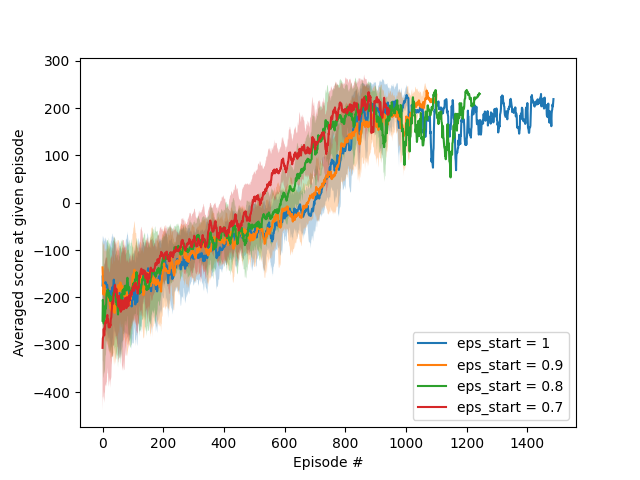
\includegraphics[width=0.8\linewidth]{figs/EPS_START.png}
%     \caption{Influence of $\varepsilon$-start on score gained by the agent during the episode. All other parameters remaining standard.}
%     \label{fig:start}
% \end{figure}

% \begin{figure}
%     \centering
%     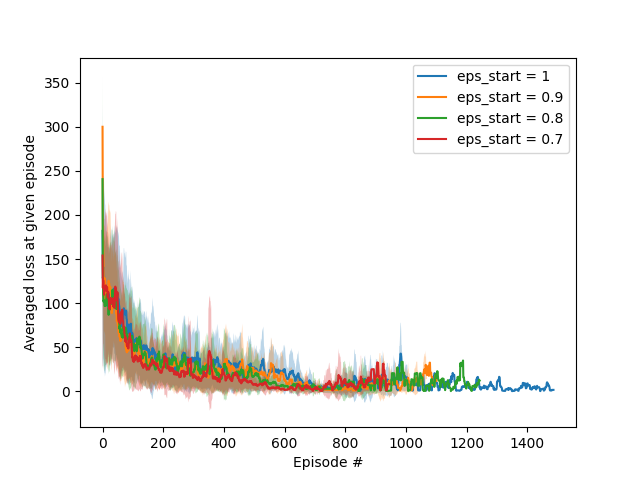
\includegraphics[width=0.8\linewidth]{figs/EPS_START(loss).png}
%     \caption{Influence of $\varepsilon$-start on score gained by the agent during the episode. All other parameters remaining standard.}
%     \label{fig:start_loss}
% \end{figure}

% \begin{figure}
%     \centering
%     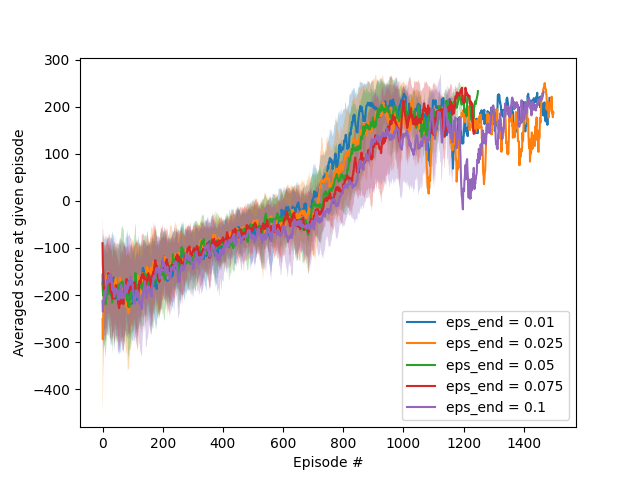
\includegraphics[width=0.8\linewidth]{figs/EPS_END.png}
%     \caption{Influence of $\varepsilon$-end on score gained by the agent during the episode. All other parameters remaining standard.}
%     \label{fig:end}
% \end{figure}

% \begin{figure}
%     \centering
%     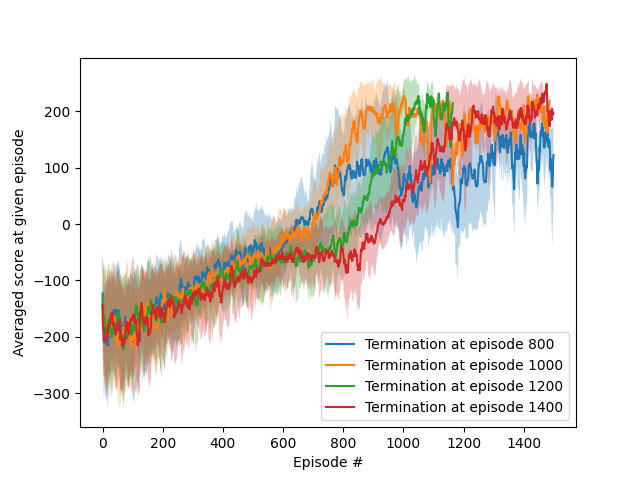
\includegraphics[width=0.8\linewidth]{figs/EPS_TERM.png}
%     \caption{Influence of $\varepsilon$-term on score gained by the agent during the episode. All other parameters remaining standard.}
%     \label{fig:term}
% \end{figure}

% \begin{figure}
%     \centering
%     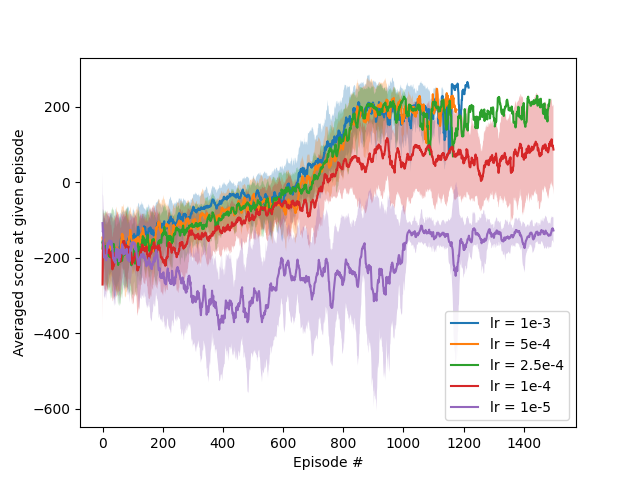
\includegraphics[width=0.8\linewidth]{figs/LR.png}
%     \caption{Averaged scores with varied learning rate $\alpha$. All other parameters remaining standard.}
%     \label{fig:lr}
% \end{figure}

% \begin{figure}
%     \centering
%     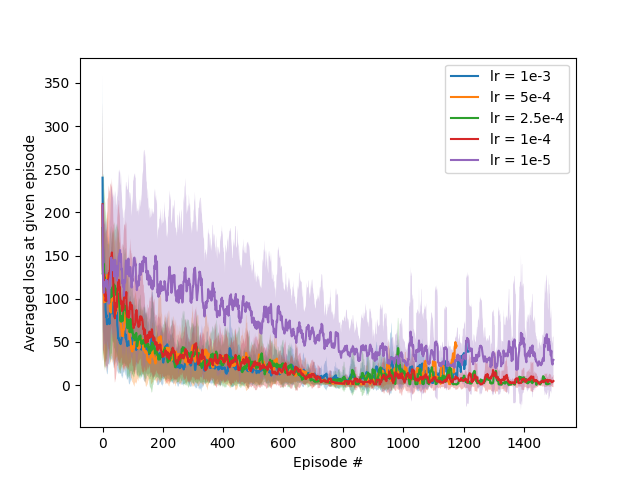
\includegraphics[width=0.8\linewidth]{figs/LR(loss).png}
%     \caption{Averaged scores with varied learning rate $\alpha$. All other parameters remaining standard.}
%     \label{fig:lr_loss}
% \end{figure}

\addcontentsline{toc}{section}{References}
\bibliographystyle{plain}
\bibliography{refs}

\end{document}